


\begin{frame}{Diploma Thesis \sof{1}{3}}

%\vspace{1em}
\justifying
My diploma thesis~\cite{Kerdels2006} presents a novel approach to {\bf discover 
objects in unlabeled image data} using a combination of traditional methods 
including image segmentation, feature extraction, clustering, and dynamic 
programming.

\vspace{1.5em}
The key idea consists of using {\bf image segmentation to group features} in an 
image, and use these feature groups to represent the individual segments in a 
way that is invariant to rotation, scale, and translation.

\vspace{1.5em}
Such feature segments can then be related to each other by an appropriate 
distance measure to {\bf identify segments that occur repeatedly} in different 
contexts.

\vspace{1.5em}
Finally, neighborhood relations among segments can be learned in a similar 
fashion to {\bf discover stable feature segment constellations} that indicate 
the presence of reoccuring structures, i.e., putative objects in the images.

\begin{center}
\rule{2cm}{0.4pt}\\[0.5em]
\end{center}

\fc{Kerdels2006}{publications/2006-01/2006-01}

\end{frame}



\begin{frame}{Diploma Thesis \sof{2}{3}}

%\vspace{1em}
\justifying

\vspace{2em}
In~\cite{Peters2007} we present details of the {\bf image 
segmentation} algorithm that was first introduced in my diploma thesis.

\vspace{1em}
The algorithm has a focus on {\bf robustness with respect to noise and 
discontinuous structures} like tree foliage. 

\vspace{1em}
\begin{figure}
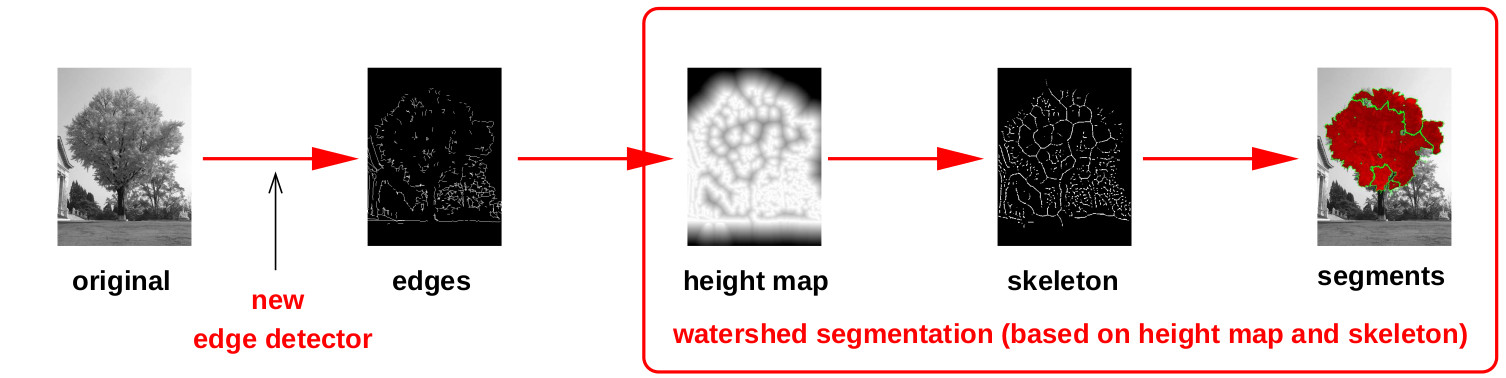
\includegraphics[width=0.66\linewidth]{diploma_thesis/segmentation.jpg}

\vspace{-0.75em}
\caption{\scriptsize Overview of the segmentation algorithm~\cite{Peters2007}.}
\end{figure}

The algorithm was featured on the cover of ``Informatik 
Spektrum''~\cite{Kerdels2007}, the main organ of the German Informatics 
Society~(GI).

\begin{center}
\rule{2cm}{0.4pt}\\[0.5em]
\end{center}

\fc{Peters2007}{publications/2007-03/2007-03}\\[1em]
\fc{Kerdels2007}{publications/2007-06/2007-06}

\end{frame}



\begin{frame}{Diploma Thesis \sof{3}{3}}

\twocol{0.25}{
\vspace{-2.5em}
\begin{figure}
\adjincludegraphics[width=1.\linewidth,valign=t]{diploma_thesis/dist_graph.jpg}
\vspace{-1em}
\caption{\scriptsize Illustration of distances on a learned 
topology~\cite{Kerdels2007a}.}
\adjincludegraphics[width=1.\linewidth,valign=b]{diploma_thesis/dist_ex.jpg}
\vspace{-1.5em}
\caption{\justifying\scriptsize Classification of feature vectors into 8 pairwise 
neighboring nodes. Columns represent nodes. Each column contains examples of 10 
feature vectors mapped onto the respective node~\cite{Kerdels2007a}.}
\end{figure}
}{0.7}{
\justifying

\vspace{1em}
In~\cite{Kerdels2007a} we present details of the {\bf feature similarity 
measure} that was first introduced in my diploma thesis. The measure utilizes
a {\bf learned topology} of the feature space and does not rely on distance in 
Euclidean space.

\vspace{2em}
Key ideas:
\begin{itemize}
	\item Utilize a growing neural gas (GNG) to learn a piecewise representation
	of the feature space as well as its topology.
	\item Determine the shortest path between all pairs of nodes in the 
	topology. 
	\item The (dis)similarity between two features \(f_1\) and \(f_2\) is then given 
	as the shortest path between those nodes \(g_1\) and \(g_1\) onto which the
	features are mapped by the GNG. 
\end{itemize}

}

\vspace{-1em}

\begin{center}
\rule{2cm}{0.4pt}\\[0.5em]
\end{center}

\fc{Kerdels2007a}{publications/2007-04/2007-04}

\end{frame}

